\documentclass[conference]{IEEEtran}
\IEEEoverridecommandlockouts
\usepackage{cite}
\usepackage{amsmath,amssymb,amsfonts}
\usepackage{algorithmic}
\usepackage{graphicx}
\usepackage{textcomp}
\usepackage{xcolor}

\def\BibTeX{{\rm B\kern-.05em{\sc i\kern-.025em b}\kern-.08em
    T\kern-.1667em\lower.7ex\hbox{E}\kern-.125emX}}
\begin{document}

\title{Otimização de Funções Custo/Objetivo em Algoritmos Meta-heurísticos}

\author{\IEEEauthorblockN{1\textsuperscript{st} Samuel Façanha Martins}
\IEEEauthorblockA{\textit{Ciências da Computação} \\
\textit{Unifor}\\
Fortaleza, CE \\
samuelfacanha@edu.unifor.br}
% Repita conforme necessário para outros autores
}

\maketitle

\begin{abstract}
Este documento apresenta uma investigação sobre a otimização de funções de custo/objetivo utilizando algoritmos meta-heurísticos. Abordamos diversos métodos, incluindo Hill Climbing, Local Random Search, Global Random Search e Simulated Annealing, em busca de soluções ótimas ou subótimas para problemas definidos, analisando ao final qual desses algorítmos se sobressai e quais hiperparâmetros são mais eficazes.
\end{abstract}

\begin{IEEEkeywords}
Otimização, Meta-heurística, Função Custo, Algoritmos, Hill Climbing, Local Random Search, Global Random Search, Simulated Annealing
\end{IEEEkeywords}

\section{Introdução}
Este estudo foca na análise de estratégias de otimização para minimização ou maximização de funções custo/objetivo. Algoritmos meta-heurísticos são explorados para encontrar soluções ótimas ou subótimas, considerando a complexidade e as restrições inerentes a esses problemas. 

\section{Fundamentação Teórica}
Os algoritmos meta-heurísticos são métodos de busca que procuram soluções ótimas para problemas de otimização. Estes problemas são caracterizados por uma função objetivo, um conjunto de variáveis independentes e um conjunto de restrições. O foco está em minimizar ou maximizar a função objetivo, respeitando as restrições impostas.

\section{Metodologia}
A metodologia envolve a aplicação dos algoritmos Hill Climbing, Local Random Search, Global Random Search e Simulated Annealing. Cada algoritmo é testado em 100 rodadas, armazenando a solução obtida a cada rodada. Os hiperparâmetros específicos de cada algoritmo são ajustados para identificar o menor valor que encontra a solução ótima. Os códigos encontram-se em anexo ao documento, e disponíveis no repositório \textit{https://github.com/samufacanha2/genetic-agorithms}.

\section{Resultados}
Os resultados incluem uma tabela com a moda das soluções de cada algoritmo. Observou-se que diferentes algoritmos e hiperparâmetros apresentam variações significativas na eficácia da otimização.

\begin{figure}
    \centering
    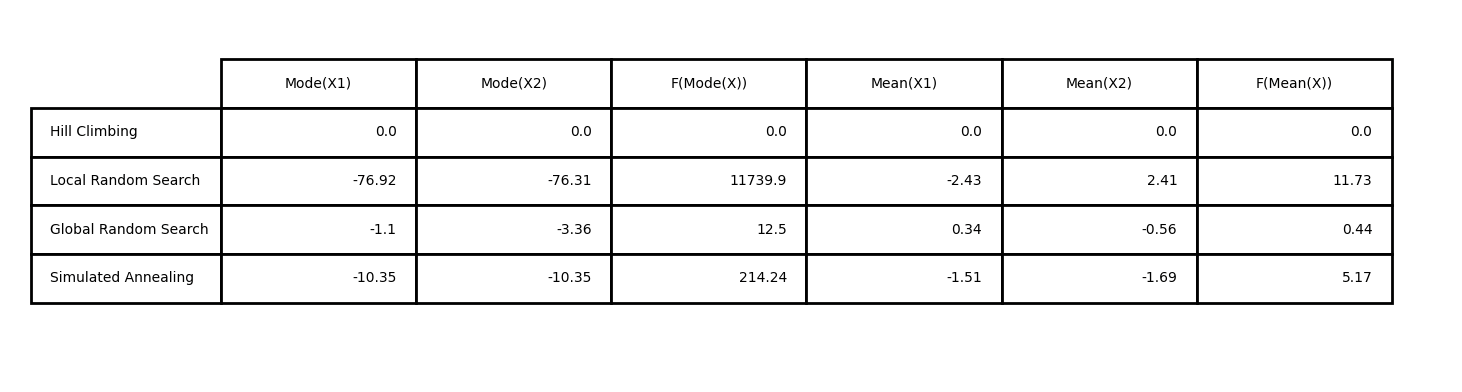
\includegraphics[width=0.5\linewidth]{images/f_1.png}
    \caption{Função 1}
    \label{fig:my_label}
\end{figure}

para a função 1, além da moda, foi calculada também a média das soluções. A média é uma medida mais robusta, pois não é afetada por outliers e pela discretização dos valores. Como essa função apresenta um mínimo global, o Hill Climbing se destaca.

\begin{figure}
    \centering
    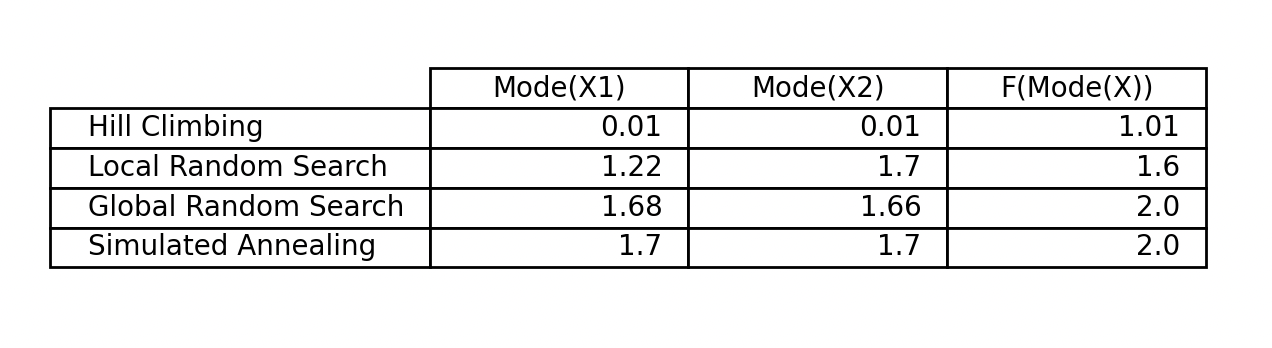
\includegraphics[width=0.5\linewidth]{images/f_2.png}
    \caption{Função 2}
    \label{fig:my_label}
\end{figure}

A função 2 apresenta dois possíveis máximos locais, e o Hill Climbing não consegue escapar de um deles, que não é o máximo global (pois sempre começa em um ponto predefinido como o de menor x1 e x2). O Simulated Annealing e o Global Random Search se destacam, pois conseguem escapar de máximos locais.

\begin{figure}
    \centering
    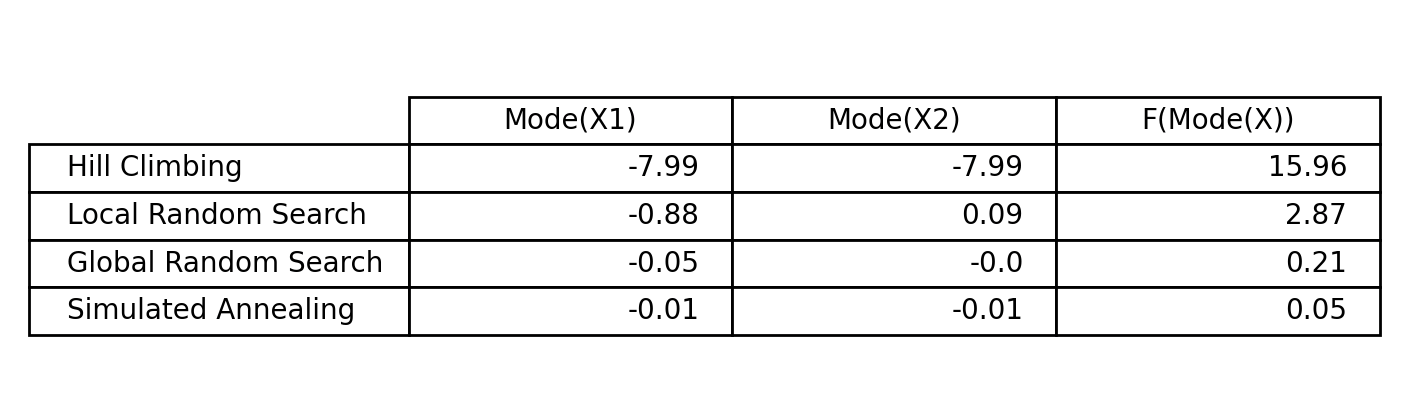
\includegraphics[width=0.5\linewidth]{images/f_3.png}
    \caption{Função 3}
    \label{fig:my_label}
\end{figure}

\begin{figure}
    \centering
    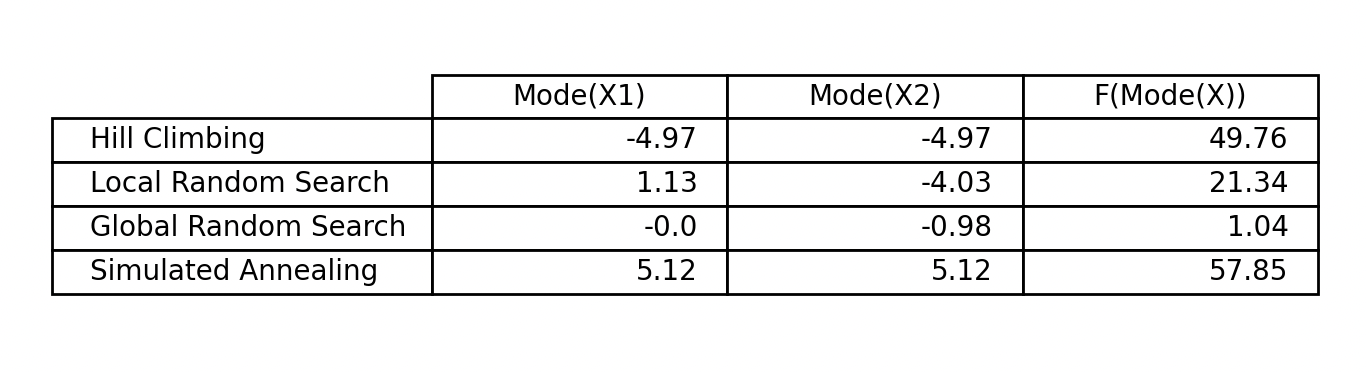
\includegraphics[width=0.5\linewidth]{images/f_4.png}
    \caption{Função 4}
    \label{fig:my_label}
\end{figure}

\begin{figure}
    \centering
    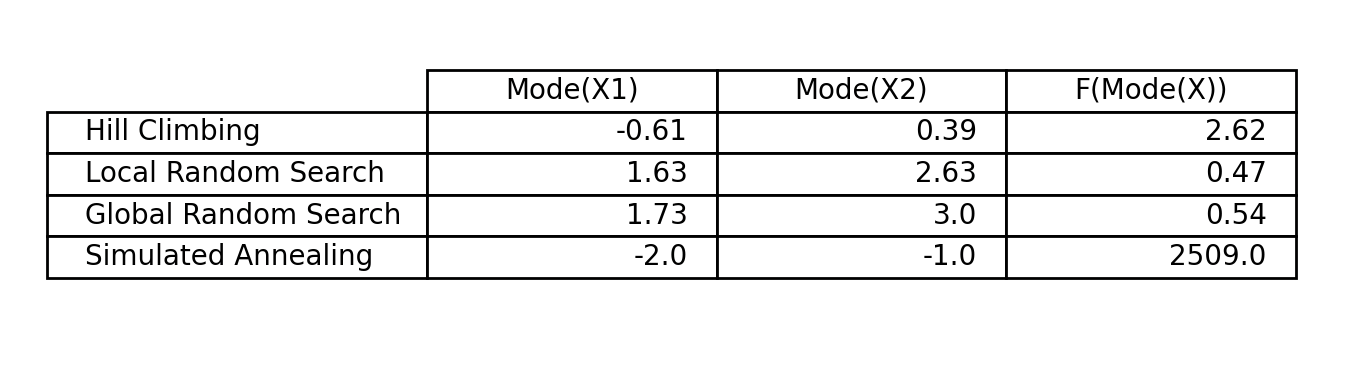
\includegraphics[width=0.5\linewidth]{images/f_5.png}
    \caption{Função 5}
    \label{fig:my_label}
\end{figure}

\begin{figure}
    \centering
    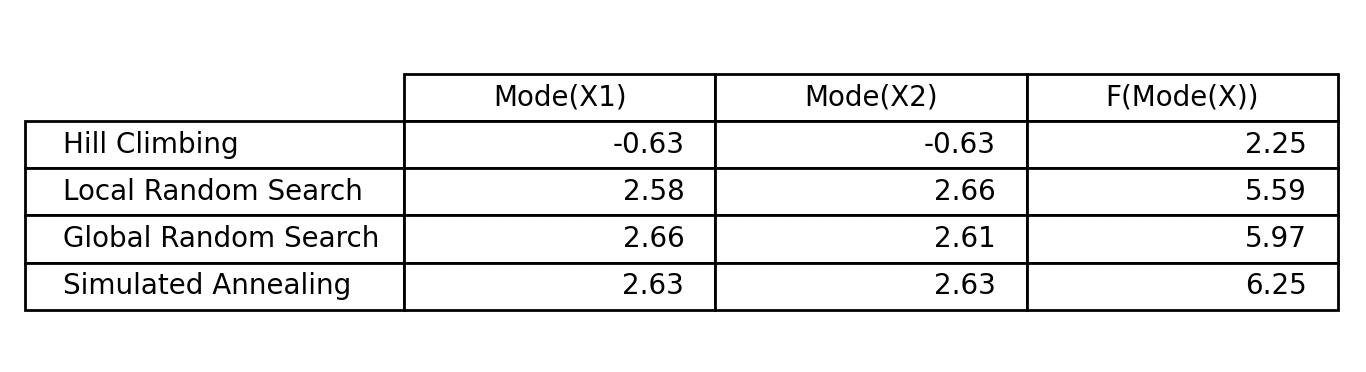
\includegraphics[width=0.5\linewidth]{images/f_6.png}
    \caption{Função 6}
    \label{fig:my_label}
\end

\begin{figure}
    \centering
    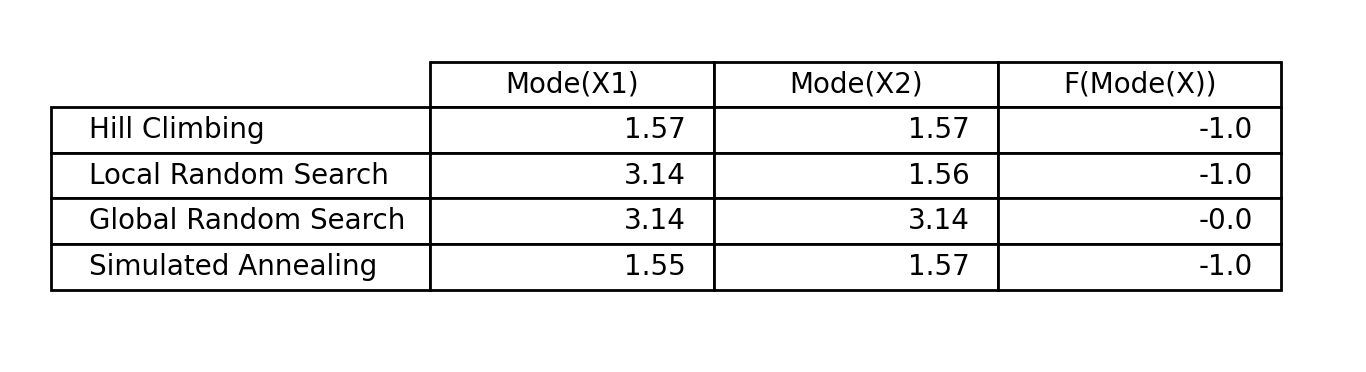
\includegraphics[width=0.5\linewidth]{images/f_7.png}
    \caption{Função 7}
    \label{fig:my_label}
\end

\begin{figure}
    \centering
    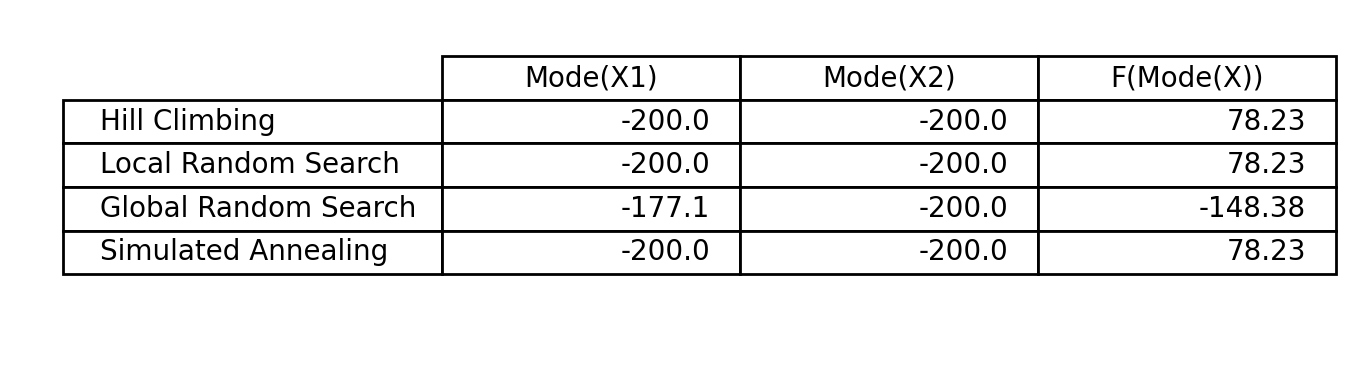
\includegraphics[width=0.5\linewidth]{images/f_8.png}
    \caption{Função 8}
    \label{fig:my_label}
\end


As funções 3, 4, 5, 6, 7 e 8 apresentam diversos máximos e mínimos locais, e o Hill Climbing em geral não consegue escapar de nenhum deles. O Simulated Annealing e o Global Random Search se destacam, pois conseguem escapar de máximos e mínimos locais. Em alguns o Local Random Search também se destaca, a depender da topologia, mas em outros não.

O maior desafio da análise dessas últimas funções é a definição dos hiperparâmetros.

\section{Conclusões}
(Espaço reservado para as conclusões após a análise dos resultados do experimento.)

\section{Referências}
(Espaço para a bibliografia.)

\end{document}
